
%(BEGIN_QUESTION)
% Copyright 2010, Tony R. Kuphaldt, released under the Creative Commons Attribution License (v 1.0)
% This means you may do almost anything with this work of mine, so long as you give me proper credit

A PLC is used to control the starting and stopping of an air compressor:

$$\includegraphics[width=15.5cm]{i02256x01.eps}$$

Suppose the electrical contact on the control switch (trip pressure = 87 PSI) corrodes, such that it cannot form a good connection when it's supposed to close.  Explain how this will affect the operation of this system, and also how you could diagnose the problem by viewing the indicator LEDs on the PLC, as well as by monitoring the ``live'' contact status in the Ladder Diagram with a laptop computer.

\vfil 

\underbar{file i02256}
\eject
%(END_QUESTION)





%(BEGIN_ANSWER)

This is a graded question -- no answers or hints given!

%(END_ANSWER)





%(BEGIN_NOTES)

If the control switch contact fails open, the PLC will ``think'' the control switch is telling it the pressure is always less than 87 PSI, because that pressure switch has a normally-open contact.  In other words, lack of power sent to the PLC input is supposed to mean ``low pressure,'' and so a broken wire connection will always send a ``low pressure'' signal to the PLC (the normally-closed X6 instruction in the PLC program will always be colored).

This does not mean that the compressor motor will run continuously, however.  If the Cut-out switch still functions as it should, input X1 will de-energize when the air pressure exceeds 102 PSI, un-coloring the X1 contact instruction in the PLC program and therefore cutting off power to the Y2 output which controls the compressor motor.  As soon as the air pressure drops down far enough to re-close the Cut-out switch's contact, though, the compressor will start right back up.

\vskip 10pt

A pithy way to summarize this state of affairs is to say that {\it the system outwardly functions as though it's been placed in ``Hand'' mode.}

\vskip 10pt

This problem will be evident as the Cut-out switch cycles (X1 indicator LED turning on and off) while the X6 indicator LED never lights up.  It will also be evident as the normally-closed virtual contact for X6 in the PLC program always remains colored, even as the virtual contact for X1 alternately colors and un-colors to start and stop the compressor.

%INDEX% PLC, troubleshooting: compressor control system, response to faulted switch
%INDEX% Process: air compressor and receiver tank

%(END_NOTES)

